% =============================================================
% Supplementary material (draft) -- BCS-Regions paper
% =============================================================
\clearpage
\section*{Supplementary material}
\setcounter{table}{0}\setcounter{figure}{0}
\renewcommand{\thetable}{S\arabic{table}}\renewcommand{\thefigure}{S\arabic{figure}}

\begin{table*}[h]
  \centering
  \caption{BCS-Regions against the baselines, split by cow (15 folds: five folds $\times$ 3 seeds; each image's prediction averaged over the seeds). $\Delta$: per-cow MAE of the baseline minus that of BCS-Regions, with a paired bootstrap 95\% CI over cows; positive means the baseline is worse. Bias: mean signed error for thin ($<3$) and fat ($\geq4.5$) cows.}
  \label{tab:S1}
  \begin{tabular}{lcccccccc}
    \toprule
    Method & MAE & RMSE & $R^2$ & $\pm0.5$ & MAE/cow & $\Delta$ MAE/cow [95\% CI] & Bias thin & Bias fat \\
    \midrule
    BCS-Regions & \textbf{0.458} & \textbf{0.565} & \textbf{0.68} & \textbf{73\%} & \textbf{0.443} & -- & \textbf{+0.61} & \textbf{$-$0.36} \\
    DINOv3 + LoRA & 0.505 & 0.639 & 0.59 & 68\% & 0.455 & +0.012 [$-$0.037, +0.057] & +0.70 & $-$0.42 \\
    ResNet-50, frozen + ridge & 0.676 & 0.840 & 0.29 & 52\% & 0.656 & +0.213 [+0.138, +0.289] & +0.86 & $-$0.74 \\
    ResNet-50, fine-tuned & 0.726 & 0.880 & 0.22 & 47\% & 0.650 & +0.207 [+0.132, +0.282] & +1.10 & $-$0.70 \\
    ViT-B/16, fine-tuned & 0.750 & 0.895 & 0.20 & 43\% & 0.669 & +0.225 [+0.152, +0.301] & +1.04 & $-$0.77 \\
    EfficientNet-V2-S, fine-tuned & 0.747 & 0.878 & 0.23 & 45\% & 0.674 & +0.231 [+0.161, +0.304] & +1.16 & $-$0.70 \\
    EfficientNet-B0, fine-tuned & 0.766 & 0.907 & 0.17 & 44\% & 0.687 & +0.243 [+0.169, +0.319] & +1.22 & $-$0.72 \\
    YOLOv8s-cls & 0.801 & 0.946 & 0.10 & 44\% & 0.701 & +0.258 [+0.167, +0.347] & +1.19 & $-$0.78 \\
    YOLO11s-cls & 0.798 & 0.970 & 0.06 & 46\% & 0.707 & +0.264 [+0.169, +0.360] & +1.30 & $-$0.69 \\
    \bottomrule
  \end{tabular}
\end{table*}

\begin{figure*}[h]
  \centering
  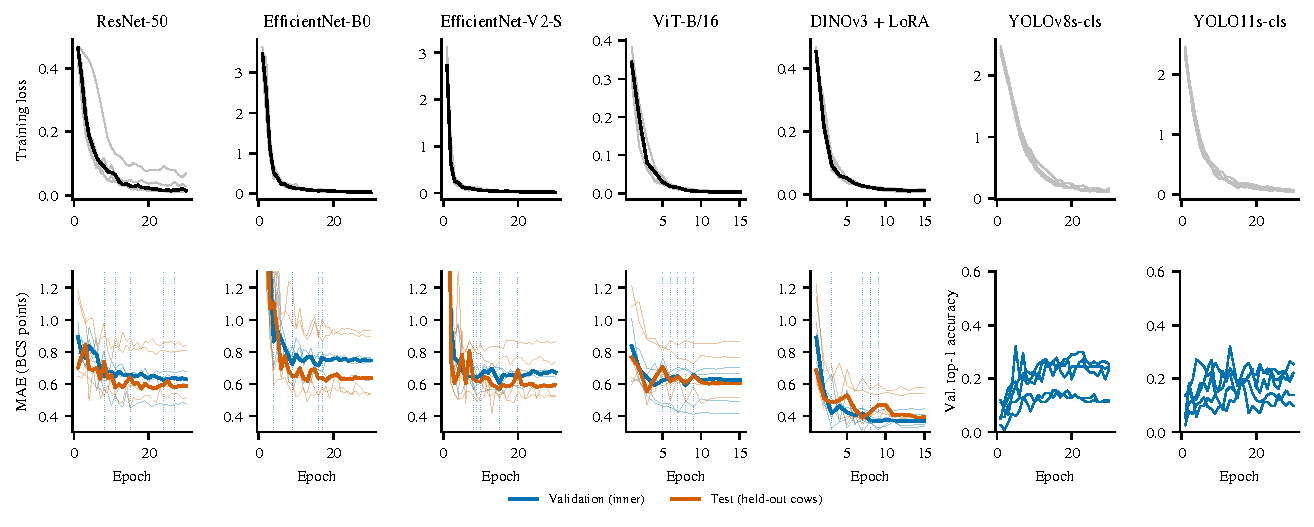
\includegraphics[width=\textwidth]{../figures/curvas_entrenamiento.pdf}
  \caption{Training curves of the fine-tuned baselines (seed 0, five cow-level folds, learning rate chosen by inner validation). Top: training loss. Bottom: MAE on the inner validation cows (blue, used to choose the epoch; dotted lines mark the chosen epochs) and on the held-out test cows (orange, shown only for reference). YOLO classifiers: validation top-1 accuracy over the 13 BCS classes. Thin lines: folds; thick lines: median over folds.}
  \label{fig:S1}
\end{figure*}

\begin{figure*}[h]
  \centering
  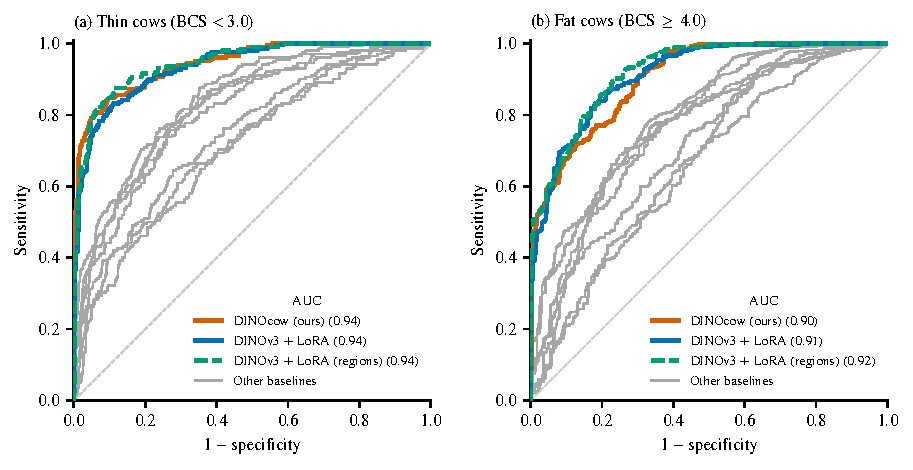
\includegraphics[width=\textwidth]{../figures/roc.pdf}
  \caption{ROC curves for flagging (a) thin (BCS $<3$) and (b) fat (BCS $\geq4$) cows with the predicted score (15 cow-level folds; prediction averaged over seeds). Areas under the curve are given in the legend and in Table~\ref{tab:summary}.}
  \label{fig:S2}
\end{figure*}

\pendiente{Fig.~S3: MAE per cow against DINOv3 block (sweep over blocks 17--24).}

\begin{figure*}[h]
  \centering
  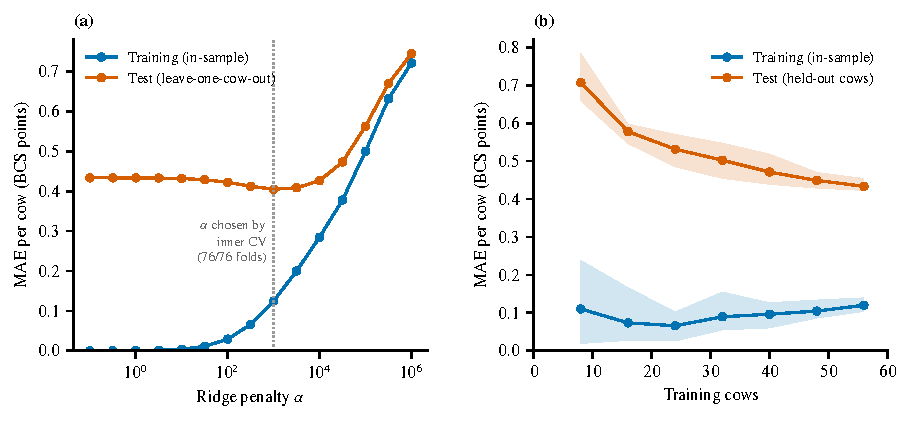
\includegraphics[width=\textwidth]{../figures/curvas_modelo.pdf}
  \caption{Training and test error of BCS-Regions. (a) MAE per cow against the ridge penalty $\alpha$ (leave-one-cow-out); the inner validation chose $\alpha = 1000$ in all 64 folds. (b) Training and test MAE per cow against the number of training cows (8 folds $\times$ 10 repetitions; bands: 2.5--97.5 percentiles).}
  \label{fig:S4}
\end{figure*}
